documentclass{beamer}
\usepackage{amsmath}
\usepackage{amsfonts}
\usepackage{amssymb}
\usepackage{graphicx}
\usepackage{tikz}
\usetikzlibrary{shapes,arrows,positioning}

\title{Hierarchical Embeddings for Disease-Signature Associations}
\subtitle{Learning Psi Parameters Through Attention Mechanisms (With much thanks to Bishop et al)}
\author{Sarah Urbut, MD PhD}



\date{\today}

\begin{document}

\frame{\titlepage}

\begin{frame}
\frametitle{Motivation: Current Psi Learning}
\begin{itemize}
\item Current approach: Learn $\psi \in \mathbb{R}^{K \times D}$ directly
\item $\psi_{k,d}$ = association strength between signature $k$ and disease $d$
\item Problems:
\begin{itemize}
\item No semantic structure between diseases
\item Difficult to generalize to new diseases
\item No interpretable disease relationships
\end{itemize}
\end{itemize}
\end{frame}

\begin{frame}
\frametitle{Simplified Hierarchical Embedding Approach}
\begin{center}
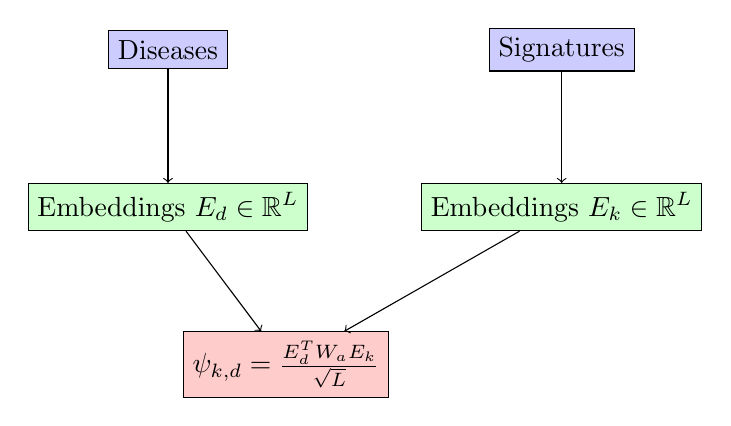
\begin{tikzpicture}[node distance=2cm]
\node (diseases) [rectangle, draw, fill=blue!20] {Diseases};
\node (embeddings) [rectangle, draw, fill=green!20, below of=diseases] {Embeddings $E_d \in \mathbb{R}^L$};
\node (signatures) [rectangle, draw, fill=green!20, right of=embeddings, xshift=3cm] {Embeddings $E_k \in \mathbb{R}^L$};
\node (sigs) [rectangle, draw, fill=blue!20, above of=signatures] {Signatures};
\node (psi) [rectangle, draw, fill=red!20, below of=embeddings, xshift=1.5cm] {$\psi_{k,d} = \frac{E_d^T W_a E_k}{\sqrt{L}}$};

\draw [->] (diseases) -- (embeddings);
\draw [->] (sigs) -- (signatures);
\draw [->] (embeddings) -- (psi);
\draw [->] (signatures) -- (psi);
\end{tikzpicture}
\end{center}
\end{frame}

\begin{frame}
\frametitle{Mathematical Formulation: Direct Approach}
\begin{block}{Step 1: Disease and Signature Embeddings}
\begin{align}
E_d &\in \mathbb{R}^L \quad \text{(disease embeddings)} \\
E_k &\in \mathbb{R}^L \quad \text{(signature embeddings)}
\end{align}
\end{block}

\begin{block}{Step 2: Direct Psi Computation}
\begin{align}
\psi_{k,d} &= \frac{E_d^T W_a E_k}{\sqrt{L}} \in \mathbb{R}
\end{align}
where $W_a \in \mathbb{R}^{L \times L}$ is learnable.
\end{block}

\begin{block}{Key Insight:}
Skip attention softmax and contextualization - use raw attention scores directly as $\psi$ values.
\end{block}
\end{frame}

\begin{frame}
\frametitle{Tensor Dimensions}
\begin{center}
\begin{tabular}{|c|c|c|}
\hline
\textbf{Variable} & \textbf{Shape} & \textbf{Description} \\
\hline
$E_d$ & $[D, L]$ & Disease embeddings \\
$E_k$ & $[K, L]$ & Signature embeddings \\
$W_a$ & $[L, L]$ & Attention interaction matrix \\
$\psi$ & $[K, D]$ & Final association strengths \\
\hline
\end{tabular}
\end{center}

\begin{itemize}
\item $D$ = number of diseases
\item $K$ = number of signatures  
\item $L$ = embedding dimension
\end{itemize}
\end{frame}

\begin{frame}
\frametitle{What Each Component Means}
\begin{block}{Disease Embeddings $E_d$:}
Each disease is represented by an $L$-dimensional vector capturing its biological characteristics.
\end{block}

\begin{block}{Signature Embeddings $E_k$:}
Each signature is represented by an $L$-dimensional vector capturing pathway characteristics.
\end{block}

\begin{block}{Attention Matrix $W_a$:}
Learns which disease features should interact with which signature features.
\end{block}

\begin{block}{Final Association $\psi_{k,d}$:}
Direct measure of how strongly disease $d$ associates with signature $k$.
\end{block}
\end{frame}

\begin{frame}
\frametitle{Implementation in PyTorch}
\begin{block}{Key Components:}
\begin{verbatim}
# Embeddings
self.disease_embeddings = nn.Embedding(D, L)
self.signature_embeddings = nn.Embedding(K, L)

# Attention interaction matrix
self.attention_matrix = nn.Parameter(torch.randn(L, L))
\end{verbatim}
\end{block}

\begin{block}{Forward Pass:}
\begin{verbatim}
def compute_psi_from_embeddings(self):
    E_d = self.disease_embeddings(torch.arange(D))  # [D, L]
    E_k = self.signature_embeddings(torch.arange(K)) # [K, L]
    
    # Direct psi computation
    psi_scores = torch.matmul(
        torch.matmul(E_d, self.attention_matrix),  # [D, L]
        E_k.T                                     # [L, K]
    ) / math.sqrt(L)  # [D, K]
    
    return psi_scores.T  # [K, D]
\end{verbatim}
\end{block}
\end{frame}



\begin{frame}
\frametitle{Implementation in PyTorch}
\begin{block}{Key Components:}
\begin{verbatim}
# Embeddings
self.disease_embeddings = nn.Embedding(D, L)
self.signature_embeddings = nn.Embedding(K, L)

# Attention and projection
self.attention_matrix = nn.Parameter(torch.randn(L, L))
self.psi_projection = nn.Linear(L, 1)
\end{verbatim}
\end{block}

\begin{block}{Forward Pass:}
\begin{verbatim}
def compute_psi_from_embeddings(self):
    E_d = self.disease_embeddings(torch.arange(D))
    E_k = self.signature_embeddings(torch.arange(K))
    
    # Attention
    # Direct psi computation
    psi_scores = torch.matmul(
        torch.matmul(E_d, self.attention_matrix),  # [D, L]
        E_k.T                                     # [L, K]
    ) / math.sqrt(L)  # [D, K]
    
    return psi_scores.T  # [K, D]
    
\end{verbatim}
\end{block}
\end{frame}

\begin{frame}
\frametitle{Advantages of Simplified Approach}
\begin{block}{Mathematical Clarity:}
\begin{itemize}
\item Direct mapping from embeddings to $\psi$ parameters
\item No unnecessary intermediate steps
\item Clear interpretation: $\psi$ measures embedding compatibility
\end{itemize}
\end{block}

\begin{block}{Parameter Efficiency:}
\begin{itemize}
\item Direct: $O(D \times K)$ parameters
\item Simplified Hierarchical: $O(D \times L + K \times L + L^2)$ parameters
\item No additional projection layers needed
\end{itemize}
\end{block}

\begin{block}{Easier Optimization:}
\begin{itemize}
\item Fewer parameters to learn
\item More direct gradient flow
\item Less prone to vanishing gradients
\end{itemize}
\end{block}
\end{frame}

\begin{frame}
\frametitle{Biological Interpretation}
\begin{center}
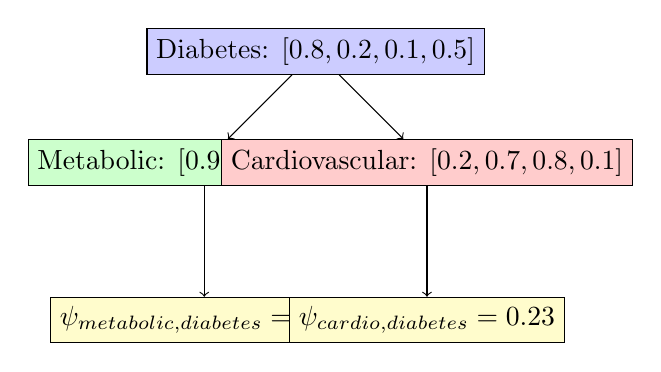
\begin{tikzpicture}[node distance=2cm]
\node (diabetes) [rectangle, draw, fill=blue!20] {Diabetes: $[0.8, 0.2, 0.1, 0.5]$};
\node (metabolic) [rectangle, draw, fill=green!20, below left of=diabetes] {Metabolic: $[0.9, 0.1, 0.0, 0.4]$};
\node (cardio) [rectangle, draw, fill=red!20, below right of=diabetes] {Cardiovascular: $[0.2, 0.7, 0.8, 0.1]$};

\node (psi1) [rectangle, draw, fill=yellow!20, below of=metabolic] {$\psi_{metabolic,diabetes} = 0.85$};
\node (psi2) [rectangle, draw, fill=yellow!20, below of=cardio] {$\psi_{cardio,diabetes} = 0.23$};

\draw [->] (diabetes) -- (metabolic);
\draw [->] (diabetes) -- (cardio);
\draw [->] (metabolic) -- (psi1);
\draw [->] (cardio) -- (psi2);
\end{tikzpicture}
\end{center}

\begin{block}{Interpretation:}
Diabetes embedding is more compatible with metabolic signature embedding through the learned $W_a$ transformation.
\end{block}
\end{frame}

\begin{frame}
\frametitle{Extension: Medication Effects}
\begin{block}{Medication-Aware Embeddings:}
\begin{align}
E_d(m) &= E_d^{base} + E_d^{med} \cdot m_d \\
E_k(m) &= E_k^{base} + E_k^{med} \cdot m_k
\end{align}
where $m_d, m_k$ are medication status indicators.
\end{block}

\begin{block}{Medication-Aware Psi:}
\begin{align}
\psi_{k,d}(m) &= \frac{E_d(m)^T W_a E_k(m)}{\sqrt{L}} + W_{med}^T m_d
\end{align}
\end{block}

\begin{block}{Benefits:}
\begin{itemize}
\item Direct medication effects on embeddings
\item Learns how treatments modify disease-signature associations
\item Maintains mathematical simplicity
\end{itemize}
\end{block}
\end{frame}

\begin{frame}
\frametitle{Loss Function}
\begin{block}{Total Loss:}
\begin{align}
L_{total} &= L_{data} + \lambda_{gp} L_{gp} + \lambda_{emb} L_{emb}
\end{align}
\end{block}

\begin{block}{Regularization Terms:}
\begin{align}
L_{emb} &= ||E_d||_2^2 + ||E_k||_2^2 + ||W_a||_2^2
\end{align}
\end{block}

\begin{block}{Simplified Gradient Flow:}
\begin{align}
\frac{\partial L}{\partial \psi} \rightarrow \frac{\partial L}{\partial E_d}, \frac{\partial L}{\partial E_k}, \frac{\partial L}{\partial W_a}
\end{align}
\end{block}

\begin{block}{Key Advantage:}
Direct gradient flow from loss to all parameters - no complex chain rule through contextualization.
\end{block}
\end{frame}

\begin{frame}
\frametitle{Key Benefits}
\begin{block}{Semantic Structure:}
\begin{itemize}
\item Diseases with similar embeddings have similar $\psi$ values
\item Learned relationships are directly interpretable
\item $W_a$ reveals which features interact across diseases and signatures
\end{itemize}
\end{block}

\begin{block}{Model-Based Approach:}
\begin{itemize}
\item Maintains principled probabilistic framework
\item Embeddings provide regularization through shared representations
\item Can incorporate external knowledge (medical ontologies, etc.)
\end{itemize}
\end{block}

\begin{block}{Practical Advantages:}
\begin{itemize}
\item Easier to implement and debug
\item Faster training with fewer parameters
\item More stable optimization
\end{itemize}
\end{block}
\end{frame}

\begin{frame}
\frametitle{Comparison: Complex vs Simplified}
\begin{center}
\begin{tabular}{|l|c|c|}
\hline
\textbf{Aspect} & \textbf{Complex (with C)} & \textbf{Simplified} \\
\hline
Steps & 4 & 2 \\
Parameters & $D \cdot L + K \cdot L + L^2 + L + 1$ & $D \cdot L + K \cdot L + L^2$ \\
Gradient Path & Long chain rule & Direct \\
Interpretability & Confusing & Clear \\
Training Stability & Lower & Higher \\
\hline
\end{tabular}
\end{center}

\begin{block}{Recommendation:}
Use the simplified approach unless you have a specific need for the contextualization step.
\end{block}
\end{frame}

\begin{frame}
\frametitle{Summary}
\begin{block}{What We've Done:}
\begin{itemize}
\item Simplified hierarchical embeddings by removing contextualization
\item Use raw attention scores directly as $\psi$ parameters
\item Maintained all benefits: semantic structure, generalization, efficiency
\item Improved optimization and interpretability
\end{itemize}
\end{block}

\begin{block}{Key Insight:}
$\psi_{k,d} = E_d^T W_a E_k$ directly captures disease-signature compatibility without unnecessary complexity.
\end{block}

\begin{block}{Next Steps:}
\begin{itemize}
\item Implement simplified version in existing model
\item Compare performance against complex version
\item Test on real datasets
\end{itemize}
\end{block}
\end{frame}

\end{document}